\documentclass{standalone}
\usepackage{tikz}
\usetikzlibrary{patterns, positioning}


\begin{document}
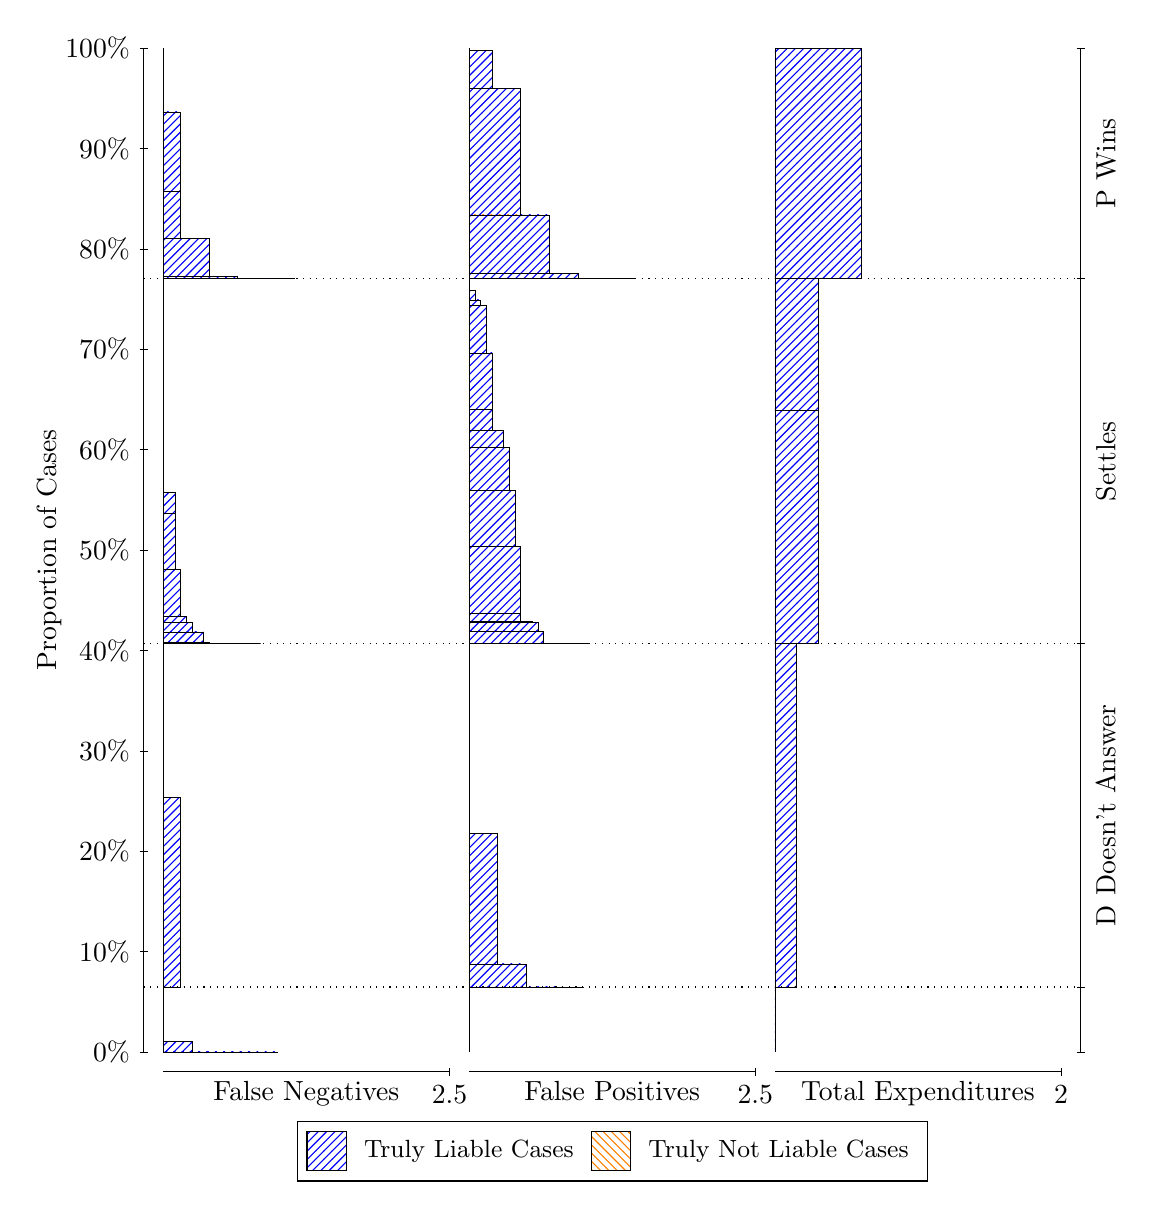
\begin{tikzpicture}
\draw[black, very thin] (1.5,1.75) -- (1.5,14.5);
\node[rotate=90, text=black, anchor=center] at (0.3, 8.125) {Proportion of Cases};
\draw[black, very thin] (1.45,1.75) -- (1.55,1.75);
\node[text=black, anchor=east] at (1.45, 1.75) {0\%};
\draw[black, very thin] (1.45,3.025) -- (1.55,3.025);
\node[text=black, anchor=east] at (1.45, 3.025) {10\%};
\draw[black, very thin] (1.45,4.3) -- (1.55,4.3);
\node[text=black, anchor=east] at (1.45, 4.3) {20\%};
\draw[black, very thin] (1.45,5.575) -- (1.55,5.575);
\node[text=black, anchor=east] at (1.45, 5.575) {30\%};
\draw[black, very thin] (1.45,6.85) -- (1.55,6.85);
\node[text=black, anchor=east] at (1.45, 6.85) {40\%};
\draw[black, very thin] (1.45,8.125) -- (1.55,8.125);
\node[text=black, anchor=east] at (1.45, 8.125) {50\%};
\draw[black, very thin] (1.45,9.4) -- (1.55,9.4);
\node[text=black, anchor=east] at (1.45, 9.4) {60\%};
\draw[black, very thin] (1.45,10.675) -- (1.55,10.675);
\node[text=black, anchor=east] at (1.45, 10.675) {70\%};
\draw[black, very thin] (1.45,11.95) -- (1.55,11.95);
\node[text=black, anchor=east] at (1.45, 11.95) {80\%};
\draw[black, very thin] (1.45,13.225) -- (1.55,13.225);
\node[text=black, anchor=east] at (1.45, 13.225) {90\%};
\draw[black, very thin] (1.45,14.5) -- (1.55,14.5);
\node[text=black, anchor=east] at (1.45, 14.5) {100\%};

\draw[black, very thin] (13.4,1.75) -- (13.4,14.5);
\draw[black, very thin] (13.35,1.75) -- (13.45,1.75);
\node[anchor=west] at (13.35, 1.75) {};
\draw[black, very thin] (13.35,2.5748) -- (13.45,2.5748);
\node[anchor=west] at (13.35, 2.5748) {};
\draw[black, very thin] (13.35,6.9363) -- (13.45,6.9363);
\node[anchor=west] at (13.35, 6.9363) {};
\draw[black, very thin] (13.35,11.571) -- (13.45,11.571);
\node[anchor=west] at (13.35, 11.571) {};
\draw[black, very thin] (13.35,14.5) -- (13.45,14.5);
\node[anchor=west] at (13.35, 14.5) {};

\draw[black, very thin, pattern color=blue, pattern=north east lines] (1.75,1.75) rectangle (3.2033,1.75);
\draw[black, very thin, pattern color=blue, pattern=north east lines] (1.75,1.75) rectangle (2.84,1.75);
\draw[black, very thin, pattern color=blue, pattern=north east lines] (1.75,1.75) rectangle (2.4767,1.7512);
\draw[black, very thin, pattern color=blue, pattern=north east lines] (1.75,1.7512) rectangle (2.1133,1.885);
\draw[black, very thin, pattern color=orange, pattern=north west lines] (1.75,1.885) rectangle (1.75,1.885);
\draw[black, very thin, pattern color=blue, pattern=north east lines] (1.75,1.885) rectangle (1.75,2.5748);
\draw[black, very thin, pattern color=blue, pattern=north east lines] (1.75,2.5748) rectangle (1.968,4.9867);
\draw[black, very thin, pattern color=orange, pattern=north west lines] (1.75,4.9867) rectangle (1.75,4.9867);
\draw[black, very thin, pattern color=blue, pattern=north east lines] (1.75,4.9867) rectangle (1.75,6.9363);
\draw[black, very thin, pattern color=blue, pattern=north east lines] (1.75,6.9363) rectangle (2.9853,6.9363);
\draw[black, very thin, pattern color=blue, pattern=north east lines] (1.75,6.9363) rectangle (2.6947,6.9363);
\draw[black, very thin, pattern color=blue, pattern=north east lines] (1.75,6.9363) rectangle (2.622,6.9365);
\draw[black, very thin, pattern color=blue, pattern=north east lines] (1.75,6.9365) rectangle (2.404,6.9366);
\draw[black, very thin, pattern color=blue, pattern=north east lines] (1.75,6.9366) rectangle (2.3313,6.9581);
\draw[black, very thin, pattern color=blue, pattern=north east lines] (1.75,6.9581) rectangle (2.2587,7.0859);
\draw[black, very thin, pattern color=blue, pattern=north east lines] (1.75,7.0859) rectangle (2.1133,7.2054);
\draw[black, very thin, pattern color=blue, pattern=north east lines] (1.75,7.2054) rectangle (2.0407,7.2784);
\draw[black, very thin, pattern color=blue, pattern=north east lines] (1.75,7.2784) rectangle (1.968,7.8792);
\draw[black, very thin, pattern color=blue, pattern=north east lines] (1.75,7.8792) rectangle (1.8953,8.5932);
\draw[black, very thin, pattern color=blue, pattern=north east lines] (1.75,8.5932) rectangle (1.8953,8.8602);
\draw[black, very thin, pattern color=orange, pattern=north west lines] (1.75,8.8602) rectangle (1.75,8.8602);
\draw[black, very thin, pattern color=blue, pattern=north east lines] (1.75,8.8602) rectangle (1.75,11.571);
\draw[black, very thin, pattern color=blue, pattern=north east lines] (1.75,11.571) rectangle (3.4213,11.571);
\draw[black, very thin, pattern color=blue, pattern=north east lines] (1.75,11.571) rectangle (3.058,11.571);
\draw[black, very thin, pattern color=blue, pattern=north east lines] (1.75,11.571) rectangle (2.6947,11.598);
\draw[black, very thin, pattern color=blue, pattern=north east lines] (1.75,11.598) rectangle (2.3313,12.083);
\draw[black, very thin, pattern color=blue, pattern=north east lines] (1.75,12.083) rectangle (1.968,12.684);
\draw[black, very thin, pattern color=blue, pattern=north east lines] (1.75,12.684) rectangle (1.968,13.689);
\draw[black, very thin, pattern color=orange, pattern=north west lines] (1.75,13.689) rectangle (1.75,13.689);
\draw[black, very thin, pattern color=blue, pattern=north east lines] (1.75,13.689) rectangle (1.75,14.5);
\draw[black, very thin, pattern color=orange, pattern=north west lines] (5.6333,1.75) rectangle (5.6333,1.75);
\draw[black, very thin, pattern color=blue, pattern=north east lines] (5.6333,1.75) rectangle (5.6333,2.5748);
\draw[black, very thin, pattern color=orange, pattern=north west lines] (5.6333,2.5748) rectangle (7.0867,2.5748);
\draw[black, very thin, pattern color=blue, pattern=north east lines] (5.6333,2.5748) rectangle (7.0867,2.5748);
\draw[black, very thin, pattern color=blue, pattern=north east lines] (5.6333,2.5748) rectangle (6.7233,2.5772);
\draw[black, very thin, pattern color=blue, pattern=north east lines] (5.6333,2.5772) rectangle (6.36,2.8691);
\draw[black, very thin, pattern color=blue, pattern=north east lines] (5.6333,2.8691) rectangle (5.9967,4.5244);
\draw[black, very thin, pattern color=blue, pattern=north east lines] (5.6333,4.5244) rectangle (5.6333,6.9363);
\draw[black, very thin, pattern color=orange, pattern=north west lines] (5.6333,6.9363) rectangle (7.1593,6.9363);
\draw[black, very thin, pattern color=blue, pattern=north east lines] (5.6333,6.9363) rectangle (7.1593,6.9363);
\draw[black, very thin, pattern color=orange, pattern=north west lines] (5.6333,6.9363) rectangle (7.014,6.9363);
\draw[black, very thin, pattern color=blue, pattern=north east lines] (5.6333,6.9363) rectangle (7.014,6.9363);
\draw[black, very thin, pattern color=orange, pattern=north west lines] (5.6333,6.9363) rectangle (6.8687,6.9363);
\draw[black, very thin, pattern color=blue, pattern=north east lines] (5.6333,6.9363) rectangle (6.8687,6.9365);
\draw[black, very thin, pattern color=blue, pattern=north east lines] (5.6333,6.9365) rectangle (6.796,6.9365);
\draw[black, very thin, pattern color=blue, pattern=north east lines] (5.6333,6.9365) rectangle (6.6507,6.9373);
\draw[black, very thin, pattern color=orange, pattern=north west lines] (5.6333,6.9373) rectangle (6.578,6.9373);
\draw[black, very thin, pattern color=blue, pattern=north east lines] (5.6333,6.9373) rectangle (6.578,7.0976);
\draw[black, very thin, pattern color=blue, pattern=north east lines] (5.6333,7.0976) rectangle (6.5053,7.2104);
\draw[black, very thin, pattern color=blue, pattern=north east lines] (5.6333,7.2104) rectangle (6.4327,7.2182);
\draw[black, very thin, pattern color=blue, pattern=north east lines] (5.6333,7.2182) rectangle (6.2873,7.3229);
\draw[black, very thin, pattern color=orange, pattern=north west lines] (5.6333,7.3229) rectangle (6.2873,7.3229);
\draw[black, very thin, pattern color=blue, pattern=north east lines] (5.6333,7.3229) rectangle (6.2873,8.1715);
\draw[black, very thin, pattern color=blue, pattern=north east lines] (5.6333,8.1715) rectangle (6.2147,8.8855);
\draw[black, very thin, pattern color=blue, pattern=north east lines] (5.6333,8.8855) rectangle (6.142,9.4246);
\draw[black, very thin, pattern color=blue, pattern=north east lines] (5.6333,9.4246) rectangle (6.0693,9.6472);
\draw[black, very thin, pattern color=blue, pattern=north east lines] (5.6333,9.6472) rectangle (5.924,9.9142);
\draw[black, very thin, pattern color=blue, pattern=north east lines] (5.6333,9.9142) rectangle (5.924,10.628);
\draw[black, very thin, pattern color=blue, pattern=north east lines] (5.6333,10.628) rectangle (5.8513,11.229);
\draw[black, very thin, pattern color=blue, pattern=north east lines] (5.6333,11.229) rectangle (5.7787,11.302);
\draw[black, very thin, pattern color=blue, pattern=north east lines] (5.6333,11.302) rectangle (5.706,11.421);
\draw[black, very thin, pattern color=blue, pattern=north east lines] (5.6333,11.421) rectangle (5.6333,11.571);
\draw[black, very thin, pattern color=orange, pattern=north west lines] (5.6333,11.571) rectangle (7.7407,11.571);
\draw[black, very thin, pattern color=blue, pattern=north east lines] (5.6333,11.571) rectangle (7.7407,11.571);
\draw[black, very thin, pattern color=orange, pattern=north west lines] (5.6333,11.571) rectangle (7.3773,11.571);
\draw[black, very thin, pattern color=blue, pattern=north east lines] (5.6333,11.571) rectangle (7.3773,11.572);
\draw[black, very thin, pattern color=orange, pattern=north west lines] (5.6333,11.572) rectangle (7.014,11.572);
\draw[black, very thin, pattern color=blue, pattern=north east lines] (5.6333,11.572) rectangle (7.014,11.637);
\draw[black, very thin, pattern color=orange, pattern=north west lines] (5.6333,11.637) rectangle (6.6507,11.637);
\draw[black, very thin, pattern color=blue, pattern=north east lines] (5.6333,11.637) rectangle (6.6507,12.382);
\draw[black, very thin, pattern color=orange, pattern=north west lines] (5.6333,12.382) rectangle (6.2873,12.382);
\draw[black, very thin, pattern color=blue, pattern=north east lines] (5.6333,12.382) rectangle (6.2873,13.989);
\draw[black, very thin, pattern color=blue, pattern=north east lines] (5.6333,13.989) rectangle (5.924,14.473);
\draw[black, very thin, pattern color=blue, pattern=north east lines] (5.6333,14.473) rectangle (5.6333,14.5);
\draw[black, very thin, pattern color=orange, pattern=north west lines] (9.5167,1.75) rectangle (9.5167,1.75);
\draw[black, very thin, pattern color=blue, pattern=north east lines] (9.5167,1.75) rectangle (9.5167,2.5748);
\draw[black, very thin, pattern color=orange, pattern=north west lines] (9.5167,2.5748) rectangle (9.7892,2.5748);
\draw[black, very thin, pattern color=blue, pattern=north east lines] (9.5167,2.5748) rectangle (9.7892,6.9363);
\draw[black, very thin, pattern color=orange, pattern=north west lines] (9.5167,6.9363) rectangle (10.062,6.9363);
\draw[black, very thin, pattern color=blue, pattern=north east lines] (9.5167,6.9363) rectangle (10.062,9.8948);
\draw[black, very thin, pattern color=orange, pattern=north west lines] (9.5167,9.8948) rectangle (10.062,9.8948);
\draw[black, very thin, pattern color=blue, pattern=north east lines] (9.5167,9.8948) rectangle (10.062,11.571);
\draw[black, very thin, pattern color=orange, pattern=north west lines] (9.5167,11.571) rectangle (10.607,11.571);
\draw[black, very thin, pattern color=blue, pattern=north east lines] (9.5167,11.571) rectangle (10.607,14.5);
\draw[black, dotted] (1.5,2.5748) -- (13.4,2.5748);
\draw[black, dotted] (1.5,6.9363) -- (13.4,6.9363);
\draw[black, dotted] (1.5,11.571) -- (13.4,11.571);
\draw[black, very thin] (1.75,1.5) -- (5.3833,1.5);
\node[text=black, anchor=north] at (3.5667, 1.5) {False Negatives};
\draw[black, very thin] (5.3833,1.45) -- (5.3833,1.55);
\node[text=black, anchor=north] at (5.3833, 1.45) {2.5};

\draw[black, very thin] (5.6333,1.5) -- (9.2667,1.5);
\node[text=black, anchor=north] at (7.45, 1.5) {False Positives};
\draw[black, very thin] (9.2667,1.45) -- (9.2667,1.55);
\node[text=black, anchor=north] at (9.2667, 1.45) {2.5};

\draw[black, very thin] (9.5167,1.5) -- (13.15,1.5);
\node[text=black, anchor=north] at (11.333, 1.5) {Total Expenditures};
\draw[black, very thin] (13.15,1.45) -- (13.15,1.55);
\node[text=black, anchor=north] at (13.15, 1.45) {2};


\node[text=black, centered, rotate=90] at (13.72, 4.7555) {D Doesn't Answer};
\node[text=black, centered, rotate=90] at (13.72, 9.2537) {Settles};
\node[text=black, centered, rotate=90] at (13.72, 13.036) {P Wins};

\draw (7.449999999999999,1.5) node[draw=none] (baseCoordinate) {};
\begin{scope}[align=center]
        \matrix[scale=0.5, draw=black, below=0.5cm of baseCoordinate, nodes={draw}, column sep=0.1cm]{
            \node[rectangle, draw, minimum width=0.5cm, minimum height=0.5cm, pattern color=blue, pattern=north east lines] {}; &
            \node[draw=none, font=\small, text=black] (B) {Truly Liable Cases}; &
            \node[rectangle, draw, minimum width=0.5cm, minimum height=0.5cm, pattern color=orange, pattern=north west lines] {}; &
            \node[draw=none, font=\small, text=black] (B) {Truly Not Liable Cases}; \\
            };
\end{scope}

\end{tikzpicture}
\end{document}